\documentclass{article}
\usepackage[utf8]{inputenc}

\title{\underline{\textit{\Large{ ENDSEMESTER EE2703 - APPLIED PROGRAMMING LAB  }}}}
\author{\textit{ SHAILESH PUPALWAR, EE20B100 }}
\date{May 12, 2022}

\usepackage{natbib}
\usepackage{graphicx}
\usepackage{amsmath}
\usepackage{listings}

\begin{document}

\maketitle

\section{Abstract}
\begin{itemize}
\item To find the antenna currents in a half-wave dipole antenna using:

(i) Standard Expression.
(ii) Magnetic Vector Potential and approximating
\item To study the difference between the graphs obtained via estimation and actual values
\end{itemize}

\section{Introduction}
We have a long wire carrying a current I(z) in dipole antenna with half length 0f 50cm(=l)
so, wavelength = 2m. Next, we need to determine the currents in the two wires of the antenna. Next, we have the expressions to calculate the value of currents.
$$I = I_{m}sin(k(l-z)) $$$$  0\leq z \leq l$$


In the next process, we calculate the magnetic vector potential by approximating the integrals (in terms of summation); we next find out $P_{ij}$ and $P_{B}$.
$$A_{z,i} = \sum_{j}P_{ij}I_{j} + P_{B}I_{N} = \sum_{j}I_{j}(\frac{\mu_{0}}{4\pi}\frac{exp(-jkR_{ij})}{R_{ij}}dz'_{j})$$

$$P_{B} = \frac{\mu_{0}}{4\pi}\frac{exp(-jkR_{iN})}{R_{iN}dz'_{j}}$$

Then, we use the Ampere's circuital law to calculate $H_{\phi}$. Again, we get it in terms of some summation involving the matrices $Q_{ij}$ and $Q_{B}$. 
$$H_{\phi}(r,z_{i}) = \sum_{j}Q_{ij}J_{j} + Q_{Bi}I_{m} = -\sum_{j}P_{ij}\frac{r}{\mu_{0}}(\frac{-jk}{R_{ij}} - \frac{1}{R^2_{ij}}) + P_{B}\frac{r}{\mu_{0}}(\frac{-jk}{R_{iN}} - \frac{1}{R^2_{iN}})$$


At last we solve the matrix equation to find out the current vector \bold{J} and then find out \bold{I}.
$$MJ = QJ + Q_{B}I_{m}$$

\section{Assignment questions}

\subsection{Question-1}
According to the question, we now need to find vector $z$ and $u$. And then find the current vectors $I$ (at loactions of $z$) and $J$ (at locations of $u$) respectively.

\newline The following code snippet does the job!
\begin{verbatim}

# Defining all the given variables 

import pylab
import numpy as np

pi = np.pi 

N = 4  # Number of sections in each half section of the antenna
Im = 1.0  # Current injected into the antenna
len = 0.5  # Quarter wavelength
w_no = pi  # Wave number = (2*pi)/(lambda)
dz = len/N  # Spacing of current samples

z = np.linspace(-len,len,2*N+1) # Points at which we determine the currents.
u = np.delete(z,[0,N,2*N]) #2*(N-1) locations of unknown currents
a = 0.01 # Radius of wire
mu_0 = 4e-7*pi # Permeability of free space

\end{verbatim}
\begin{verbatim}

The values obtained after running the code are:

z = [-0.5  -0.38 -0.25 -0.12  0.    0.12  0.25  0.38  0.5 ]
u = [-0.38 -0.25 -0.12  0.12  0.25  0.38]

\end{verbatim}

\subsection{Question-2}
According to the question, we now need determine the M vector.I defined a function to determine M vector
\newline The following code snippet does the job!
\begin{verbatim}
# Defining matrix M

def M(): # Function to determine and return the matrix M.
  M = (np.identity(2*(N-1)))*(1/(2*pi*a))
  return M
M = M()

\end{verbatim}
\begin{verbatim}
The values obtained after running the code are:
M:  [[15.92  0.    0.    0.    0.    0.  ]
 [ 0.   15.92  0.    0.    0.    0.  ]
 [ 0.    0.   15.92  0.    0.    0.  ]
 [ 0.    0.    0.   15.92  0.    0.  ]
 [ 0.    0.    0.    0.   15.92  0.  ]
 [ 0.    0.    0.    0.    0.   15.92]]
\end{verbatim}

\subsection{Question-3}
According to the question, we now need determine the matrices R_z, R_u, R_in, P and PB.

\newline The following code snippet does the job!
\begin{verbatim}
# Computing vectors R_z, R_u and matrices PB, P

Z = np.meshgrid(z,z)
z_i, z_j = Z[0], Z[1]

#R_z determines distances from source and observer where source is point of wire.
R_z = np.sqrt((z_i-z_j)**2 + np.ones([2*N+1,2*N+1],dtype=complex)*(a**2))

U = np.meshgrid(u, u)
u_i, u_j = U[0], U[1]

#R_u determines distances from source and observer where observer is point where we want the field.
R_u = np.sqrt((u_i-u_j)**2 + np.ones([2*N-2,2*N-2],dtype=complex)*(a**2))

# Distances with respect to z = 0
R_in = np.delete(R_z[:][N],[N*2,0,N])  # Removing the three elements (first, middle, last) 


# P is the contribution to the vector potential due to unknown currents
P = (mu_0/(4*pi))*(np.cos(w_no*R_u)-(np.sin(w_no*R_u))*1j)*(1/R_u)*(dz)

# PB is the contribution to the vector potential due to current "In"
PB = (mu_0/(4*pi))*(np.cos(w_no*R_in)-(np.sin(w_no*R_in))*1j)*(R_in)*(dz)
\end{verbatim}
\begin{verbatim}
The values obtained after running the code are:
R_z =
[[0.01+0.j 0.13+0.j 0.25+0.j 0.38+0.j 0.5 +0.j 0.63+0.j 0.75+0.j 0.88+0.j
  1.  +0.j]
 [0.13+0.j 0.01+0.j 0.13+0.j 0.25+0.j 0.38+0.j 0.5 +0.j 0.63+0.j 0.75+0.j
  0.88+0.j]
 [0.25+0.j 0.13+0.j 0.01+0.j 0.13+0.j 0.25+0.j 0.38+0.j 0.5 +0.j 0.63+0.j
  0.75+0.j]
 [0.38+0.j 0.25+0.j 0.13+0.j 0.01+0.j 0.13+0.j 0.25+0.j 0.38+0.j 0.5 +0.j
  0.63+0.j]
 [0.5 +0.j 0.38+0.j 0.25+0.j 0.13+0.j 0.01+0.j 0.13+0.j 0.25+0.j 0.38+0.j
  0.5 +0.j]
 [0.63+0.j 0.5 +0.j 0.38+0.j 0.25+0.j 0.13+0.j 0.01+0.j 0.13+0.j 0.25+0.j
  0.38+0.j]
 [0.75+0.j 0.63+0.j 0.5 +0.j 0.38+0.j 0.25+0.j 0.13+0.j 0.01+0.j 0.13+0.j
  0.25+0.j]
 [0.88+0.j 0.75+0.j 0.63+0.j 0.5 +0.j 0.38+0.j 0.25+0.j 0.13+0.j 0.01+0.j
  0.13+0.j]
 [1.  +0.j 0.88+0.j 0.75+0.j 0.63+0.j 0.5 +0.j 0.38+0.j 0.25+0.j 0.13+0.j
  0.01+0.j]]
  
R_u =
[[0.01+0.j 0.13+0.j 0.25+0.j 0.5 +0.j 0.63+0.j 0.75+0.j]
 [0.13+0.j 0.01+0.j 0.13+0.j 0.38+0.j 0.5 +0.j 0.63+0.j]
 [0.25+0.j 0.13+0.j 0.01+0.j 0.25+0.j 0.38+0.j 0.5 +0.j]
 [0.5 +0.j 0.38+0.j 0.25+0.j 0.01+0.j 0.13+0.j 0.25+0.j]
 [0.63+0.j 0.5 +0.j 0.38+0.j 0.13+0.j 0.01+0.j 0.13+0.j]
 [0.75+0.j 0.63+0.j 0.5 +0.j 0.25+0.j 0.13+0.j 0.01+0.j]]
 
R_in =
[0.38+0.j 0.25+0.j 0.13+0.j 0.13+0.j 0.25+0.j 0.38+0.j]

P*1e8
[[124.94-3.93j   9.2 -3.83j   3.53-3.53j  -0.  -2.5j   -0.77-1.85j
   -1.18-1.18j]
 [  9.2 -3.83j 124.94-3.93j   9.2 -3.83j   1.27-3.08j  -0.  -2.5j
   -0.77-1.85j]
 [  3.53-3.53j   9.2 -3.83j 124.94-3.93j   3.53-3.53j   1.27-3.08j
   -0.  -2.5j ]
 [ -0.  -2.5j    1.27-3.08j   3.53-3.53j 124.94-3.93j   9.2 -3.83j
    3.53-3.53j]
 [ -0.77-1.85j  -0.  -2.5j    1.27-3.08j   9.2 -3.83j 124.94-3.93j
    9.2 -3.83j]
 [ -1.18-1.18j  -0.77-1.85j  -0.  -2.5j    3.53-3.53j   9.2 -3.83j
  124.94-3.93j]]
  
PB*1e8 =
[0.18-0.43j 0.22-0.22j 0.14-0.06j 0.14-0.06j 0.22-0.22j 0.18-0.43j]

\end{verbatim}

\subsection{Question-4}
According to the question, we now need determine the matrices Q and QB.

\newline The following code snippet does the job!
\begin{verbatim}
# Computing Q and QB.

# Matrix corresponding to unknown currents
Q = (a/mu_0)*(P)*((1j)*(w_no)+(1/R_u))*(1/R_u)

# Matrix corresponding to the boundary current
QB = (a/mu_0)*(PB)*((1j)*(w_no)+(1/R_in))*(1/R_in)

\end{verbatim}
\begin{lstlisting}
The values obtained after running the code are:

Q = 
[[9.952e+01-0.j 5.000e-02-0.j 1.000e-02-0.j 0.000e+00-0.j 0.000e+00-0.j
  0.000e+00-0.j]
 [5.000e-02-0.j 9.952e+01-0.j 5.000e-02-0.j 0.000e+00-0.j 0.000e+00-0.j
  0.000e+00-0.j]
 [1.000e-02-0.j 5.000e-02-0.j 9.952e+01-0.j 1.000e-02-0.j 0.000e+00-0.j
  0.000e+00-0.j]
 [0.000e+00-0.j 0.000e+00-0.j 1.000e-02-0.j 9.952e+01-0.j 5.000e-02-0.j
  1.000e-02-0.j]
 [0.000e+00-0.j 0.000e+00-0.j 0.000e+00-0.j 5.000e-02-0.j 9.952e+01-0.j
  5.000e-02-0.j]
 [0.000e+00-0.j 0.000e+00-0.j 0.000e+00-0.j 1.000e-02-0.j 5.000e-02-0.j
  9.952e+01-0.j]]
  
QB = [0.-0.j 0.-0.j 0.-0.j 0.-0.j 0.-0.j 0.-0.j]
\end{lstlisting}

\subsection{Question-5}
According to the question, we now need determine the current density vector J and currents $I_esm$, $I_asm$.I defined a function to determine M vector
\newline The following code snippet does the job!
\begin{verbatim}
# Here we are computing Estimated currents and Assumed currents.

J = np.linalg.inv(M-Q)@QB*Im
#estimated currents
I_esm = np.concatenate(([0],J[:N-1],[Im],J[N-1:],[0]))
#assumed currents
I_asm = Im*np.sin(w_no*(len-abs(z)))
\end{verbatim}
\begin{lstlisting}
The values obtained after running the code are:

I_esm = [0. 0. 0. 0. 1. 0. 0. 0. 0.]

I_asm = [0.   0.38 0.71 0.92 1.   0.92 0.71 0.38 0.  ]
\end{lstlisting}

\begin{figure}[h!]
\centering
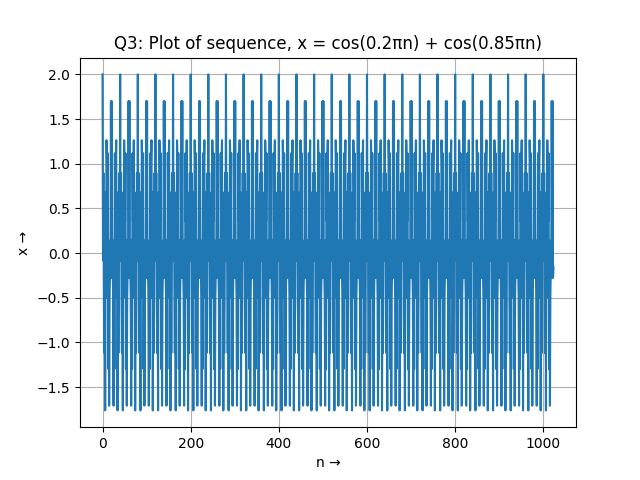
\includegraphics[scale=0.5]{Figure_1.png}
\caption{Plot of assumed current Vs estimated current}
\label{fig:universe}
\end{figure}

\begin{figure}[h!]
\centering
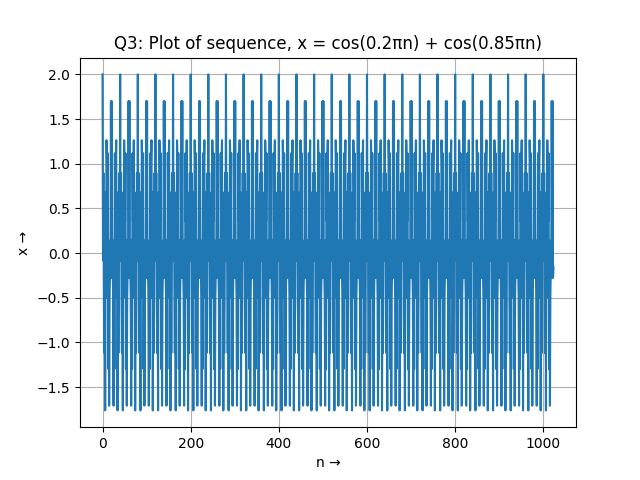
\includegraphics[scale=0.5]{Figure_2.png}
\caption{Plot of assumed current Vs estimated current}
\label{fig:universe}
\end{figure}
\newpage
\section{CONCLUSION}
\begin{itemize}
    \item On increasing the value of N,the both graph will merge each other.
    \item  On increasing N,the magnitude of point which are away from the centre
are increasing.
\end{itemize}
 \end{document}

\end{document}